\documentclass[tikz,border=3pt]{standalone}
\usepackage{xcolor}
\usetikzlibrary{arrows.meta,decorations.pathmorphing,positioning}
\definecolor{flowblue}{HTML}{2563EB}
\definecolor{retryred}{HTML}{DC2626}
\definecolor{stagefill}{HTML}{E2E8F0}
\begin{document}
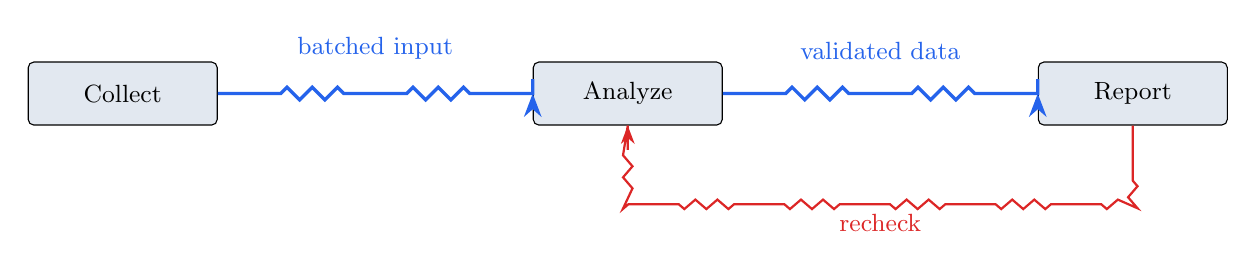
\begin{tikzpicture}[
  >=Stealth,
  stage/.style={draw,rounded corners=2pt,minimum width=2.4cm,minimum height=8mm,fill=stagefill},
  every node/.style={font=\small}
]
  \node[stage] (collect) {Collect};
  \node[stage,right=4cm of collect] (analyze) {Analyze};
  \node[stage,right=4cm of analyze] (report) {Report};
  \draw[flowblue,very thick,-Stealth,decorate,
    decoration={straight zigzag,meta-segment length=8mm,segment length=3.2mm,amplitude=.8mm}]
    (collect) -- node[above=3mm]{batched input} (analyze);
  \draw[flowblue,very thick,-Stealth,decorate,
    decoration={straight zigzag,meta-segment length=8mm,segment length=3.2mm,amplitude=.8mm}]
    (analyze) -- node[above=3mm]{validated data} (report);
  \draw[retryred,thick,-Stealth,decorate,
    decoration={straight zigzag,meta-segment length=7mm,segment length=2.8mm,amplitude=.6mm}]
    (report.south) -- ++(0,-1) -| node[below,pos=.25]{recheck} (analyze.south);
\end{tikzpicture}
\end{document}
